%% 
%% Copyright 2007, 2008, 2009 Elsevier Ltd
%% 
%% This file is part of the 'Elsarticle Bundle'.
%% ---------------------------------------------
%% 
%% It may be distributed under the conditions of the LaTeX Project Public
%% License, either version 1.2 of this license or (at your option) any
%% later version.  The latest version of this license is in
%%    http://www.latex-project.org/lppl.txt
%% and version 1.2 or later is part of all distributions of LaTeX
%% version 1999/12/01 or later.
%% 
%% The list of all files belonging to the 'Elsarticle Bundle' is
%% given in the file `manifest.txt'.
%% 

%% Template article for Elsevier's document class `elsarticle'
%% with numbered style bibliographic references
%% SP 2008/03/01

\documentclass[preprint,12pt, a4paper]{elsarticle}

%% Use the option review to obtain double line spacing
%% \documentclass[authoryear,preprint,review,12pt]{elsarticle}

%% For including figures, graphicx.sty has been loaded in
%% elsarticle.cls. If you prefer to use the old commands
%% please give \usepackage{epsfig}

%% The amssymb package provides various useful mathematical symbols
\usepackage{amssymb}
\usepackage{hyperref}
%% The amsthm package provides extended theorem environments
%% \usepackage{amsthm}

%% The lineno packages adds line numbers. Start line numbering with
%% \begin{linenumbers}, end it with \end{linenumbers}. Or switch it on
%% for the whole article with \linenumbers.
%\usepackage{lineno}

\journal{Software Impacts}

\begin{document}

\begin{frontmatter}

%% Title, authors and addresses

%% use the tnoteref command within \title for footnotes;
%% use the tnotetext command for theassociated footnote;
%% use the fnref command within \author or \address for footnotes;
%% use the fntext command for theassociated footnote;
%% use the corref command within \author for corresponding author footnotes;
%% use the cortext command for theassociated footnote;
%% use the ead command for the email address,
%% and the form \ead[url] for the home page:
%% \title{Title\tnoteref{label1}}
%% \tnotetext[label1]{}
%% \author{Name\corref{cor1}\fnref{label2}}
%% \ead{email address}
%% \ead[url]{home page}
%% \fntext[label2]{}
%% \cortext[cor1]{}
%% \address{Address\fnref{label3}}
%% \fntext[label3]{}

\title{MinViME / Minimum Viable Model Estimator}

%% use optional labels to link authors explicitly to addresses:
%% \author[label1,label2]{}
%% \address[label1]{}
%% \address[label2]{}

\author{John Hawkins}

\address{}

\begin{abstract}
%% Text of abstract 
MinViME is a python package and web application that allows scientists and engineers
to estimate a lower bound on the performance characteristics of a machine
learning model for a problem with well quantified characteristics. 

It is used to evaluate the feasibility of machine learning projects, 
prioritize among multiple competing projects, and run simulations to explore the
structure of the difficulty landscape in a multi-dimensional 
space of potential problems.

\end{abstract}

\begin{keyword}
%% keywords here, in the form: keyword \sep keyword
data science \sep machine learning \sep project management \sep estimation

%% PACS codes here, in the form: \PACS code \sep code

%% MSC codes here, in the form: \MSC code \sep code
%% or \MSC[2008] code \sep code (2000 is the default)

\end{keyword}

\end{frontmatter}

%\linenumbers

\noindent

\section{Introduction}

Machine learning projects are undertaken with an expectation
that they will add value to the process in which they will be used.
The value added depends on both the performance characteristics of the model
and the characteristics of the domain of application. These dual sets
of constraints mean that for any specific problem there is an
{\it in-principal} minimally performant model that would provide the required
value.

MinViME is a software application that allows developers and data scientists
to estimate the minimal performance characteristics of a machine learning
model for a specific application. The user enters the specification of the problem
and the costs and benefits of the decision scenario the model will assist with.
This structure follows the cost matrix analysis used in the cost sensitive learning
literature \cite{Domingos1999,Margineantu2000,Elkan2001,Tian+Zhang2019}, and
elsewhere used to adjust the decision threshold of classifier systems \cite{Nikolaou2016}
and estimate the ROI of machine learning solutions \cite{Ylijoki2018}.
 
In our theoretical work we demonstrated that the MinViME system can produce a range of metrics 
from both analytical and numerical techniques \cite{Hawkins2020}. These metrics include: 
minimal \textit{precision}, estimated \textit{AUC} and a novel \textit{simplicity}  
metric which allows for direct comparison between machine learning projects purely 
on the basis of the business criteria.

\section{Architecture}

The MinViME application consists of an underlying API that can be used inside custom
applications and simulations. The API exposes methods for generating estimated model
performance from numerical quantification of the problem.
In addition the package installs a web based graphical
used interface that is deployed as a flask application. The input screen depicted
in Figure \ref{screen1} allows a user to configure the characteristics of the business
scenario. 

\begin{figure}[h!]
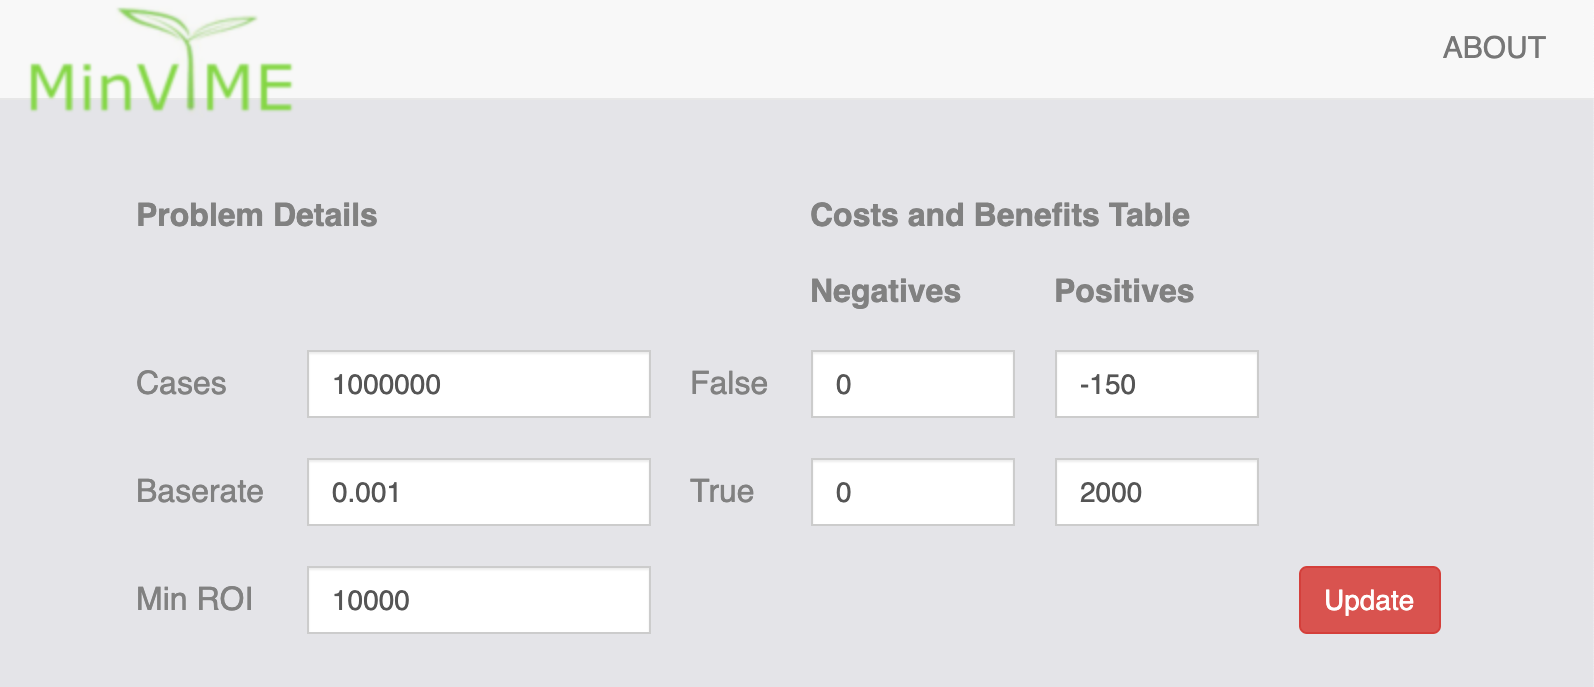
\includegraphics[scale=0.5]{images/Screen1.png}
\caption{MinViME Web Application Problem Input Screen}
\label{screen1}
\end{figure}

Upon submission, the system makes the API calls to generate analytical and
numerically simulated estimates of the minimum viable model's performance. The results
are presented as a table of metrics and plot of the estimated ROC plot (shown in Figure \ref{screen2}), which allows us to present an estimated AUC\cite{Bradley97}.
 
\begin{figure}[h!]
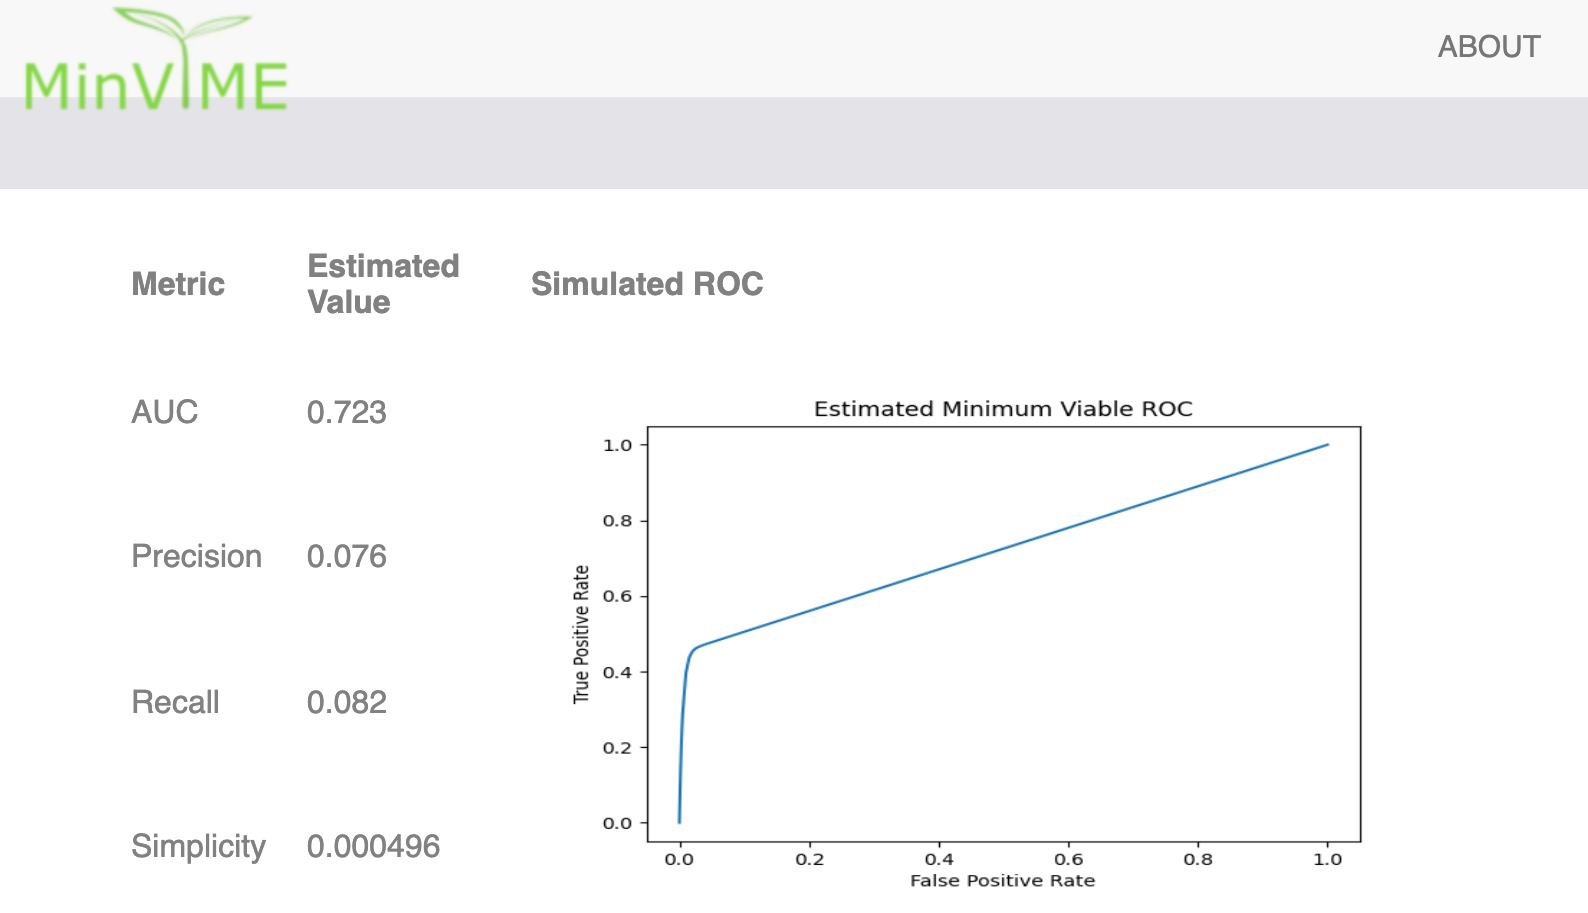
\includegraphics[scale=0.5]{images/Screen2.png}
\caption{MinViME Web Application Results Screen}
\label{screen2}
\end{figure}

\section{Impact}

The MinViME package has permitted us to run simulation experiments to answer questions
about the relationship between the landscape of business problems and the minimum 
viable models that would solve them \cite{Hawkins2020}.
These simulations form the basis of a new set of heuristics for managers of data science
and machine learning projects.

Through analysis of the PyPi package datasets (packaging.python.org)
we determined that the MinViME package has been installed 
by $>640$ users since its release 6 month ago, and the monthly downloads 
remain at $~60$ per month.


\section{Future Work}

We are currently working on extensions of the MinViME API to allow estimation of 
minimal viable models for regression and time series forecasting problems. 
This will lead to subsequent simulation work in exploring the problem difficulty landscape
for these classes of problems. 

We anticipate that these API's will find additional
utility for scientists and engineers extending the design of automated machine learning
(AutoML) \cite{zoller2021} systems so that they may determine whether the cost 
of training a model is justified by the likelihood of success.


\bibliographystyle{elsarticle-num}

\bibliography{refs}

\section*{Required Metadata}
\label{}

\section*{Current code version}
\label{}

\begin{table}[!h]
\begin{tabular}{|l|p{6.5cm}|p{6.5cm}|}
\hline
\textbf{Nr.} & \textbf{Code metadata description} & \textbf{} \\
\hline
C1 & Current code version & V1.0.0 \\
\hline
C2 & Permanent link to code/repository & https://github.com/john-hawkins/minvime \\
\hline
C3  & Permanent link to Reproducible Capsule & https://pypi.org/project/minvime/ \\
\hline
C4 & Legal Code License   & MIT \\
\hline
C5 & Code versioning system used & git \\
\hline
C6 & Software code languages, tools, and services & Python3\\
\hline
C7 & Compilation requirements, operating environments \& dependencies & Python3, Flask, numpy, pandas, matplotlib\\
\hline
C8 & If available Link to developer documentation/manual & https://minvime.readthedocs.io/ \\
\hline
C9 & Support email for questions & john@getting-data-science-done.com \\
\hline
\end{tabular}
\caption{Code metadata (mandatory)}
\label{} 
\end{table}

\end{document}
\endinput
%%
%% End of file `SoftwareX_article_template.tex'.
